%! TEX root = **/000-main.tex
% vim: spell spelllang=en:

\section{Validation protocol}%
\label{sub:validation}

\subsection{Train-Test Split}%

We separated the data into a training set and a test set before starting any analysis
into a 20\% test 80\% training data split. We decided to do the split stratified by
\texttt{league\_type}, so that the training and test had an equal balance of players from
different background.

To ensure that the split is reproducible,
we used \texttt{train\_test\_split} function with a fixed \texttt{random\_state}.

The datasets were saved in different files in \texttt{data/} directory.

%TODO: NA???????
%
\begin{table}[htb]
\centering
\caption{Train-test split}
\label{tab:train-test-split}
\begin{tabular}{lrr}
  \toprule
  \textbf{league\_type} & \textbf{Train} & \textbf{Test} \\
  \midrule
  College        &  739  & 186 \\
  NA             &  150  &  37 \\
  International  &  143  &  36 \\
  G-league       &   16  &   4 \\
  \bottomrule
\end{tabular}
\end{table}

\subsection{Cross-validation}%
\label{ssub:cross-validation}

For all the models, we used 5-fold cross validation to evaluate the performance
of the model. The same kind of 5-fold cross validation was used when doing grid
searches for parameter tuning to mitigate overfitting. As opposed to the initial
train-test split, we did not do stratification. All the cross validation steps
used a fixed random state for reproducibility.

\section{Modelling}%
\label{sub:results}

We tried several models to predict the value of our target variable. Since our target
was a numerical variable, we tried models for regression, but we also experimented with
classification models by discretizing the target variable into several categories.

\subsection{Linear Regression}%
\label{ssub:linear-regression}

As our target is continuous, our first approach was to try to solve the problem using linear regression. We started trying the Ordinary Least Squares (OLS) without much additional preprocessing and improved from there. We also tried several regularized models like Ridge which uses $L_1$ a penalty or Lasso which uses a $L_2$ penalty and ElasticNet which has a penalty that's a mix of both. For these models, we performed a grid-search cross-validation to select decent values for the penalties. Additionally, we tried using the \texttt{PolynomialFeatures} transformer with degree 2, which basically adds the degree-2 polynomial features along first the first-order interaction features.

\Cref{ml:lr} shows the results obtained with the best parameters for each algorithm we tried. One interesting detail is that OLS and Ridge performed worse when we added the 2nd degree features. This might be because most of the added features have no value.  Lasso and ElasticNet improved their results because they can set some feature coefficients to exactly zero, thus work well in highly irrelevant feature spaces. 

\begin{table}[H]
    \centering
    \begin{tabular}{lccccc}
        \toprule
        name & RMSE & $R^2$ & poly\_degree &  lr\_alpha &  l1\_ratio \\
        \midrule
        OLS & -8.258 & -2.7e+21 &       1 &        -   &        - \\
        Ridge & -8.219 &  -0.01 &        1 &       0.90 &        - \\
        Lasso & -7.962 &  0.19  &         2 &       0.45 &        - \\
        ElasticNet & -7.963 &  0.19 &      2 &       0.45 &      0.9 \\
        \bottomrule
    \end{tabular}
    \caption{Linear regression best models}
    \label{ml:lr}
\end{table}

\Cref{fig:lasso-res} shows the residuals and 

\begin{figure}[H]
    \centering
    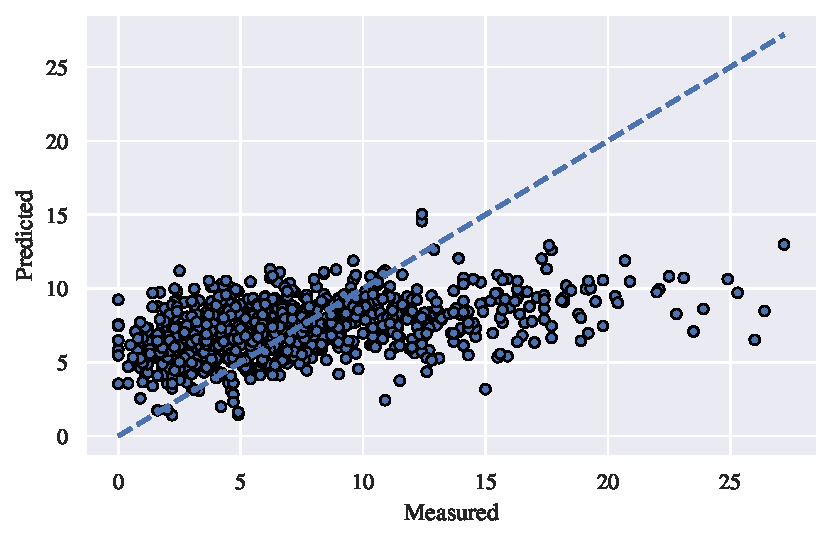
\includegraphics[width=1.0\linewidth]{figures/Lasso_residuals.pdf}
    \caption{Lasso plots}
    \label{fig:lasso-res}
\end{figure}

Moreover, we studied the coefficients of Lasso, which was our best performing model. As many features were generated, \cref{fig:lasso-coeff} only shows the coefficients with the highest absolute values. Win-shares, steals per game and points per game have high positive values, while on the other hand age and seasons played have an inverse relation to the target. 

\begin{figure}[H]
    \centering
    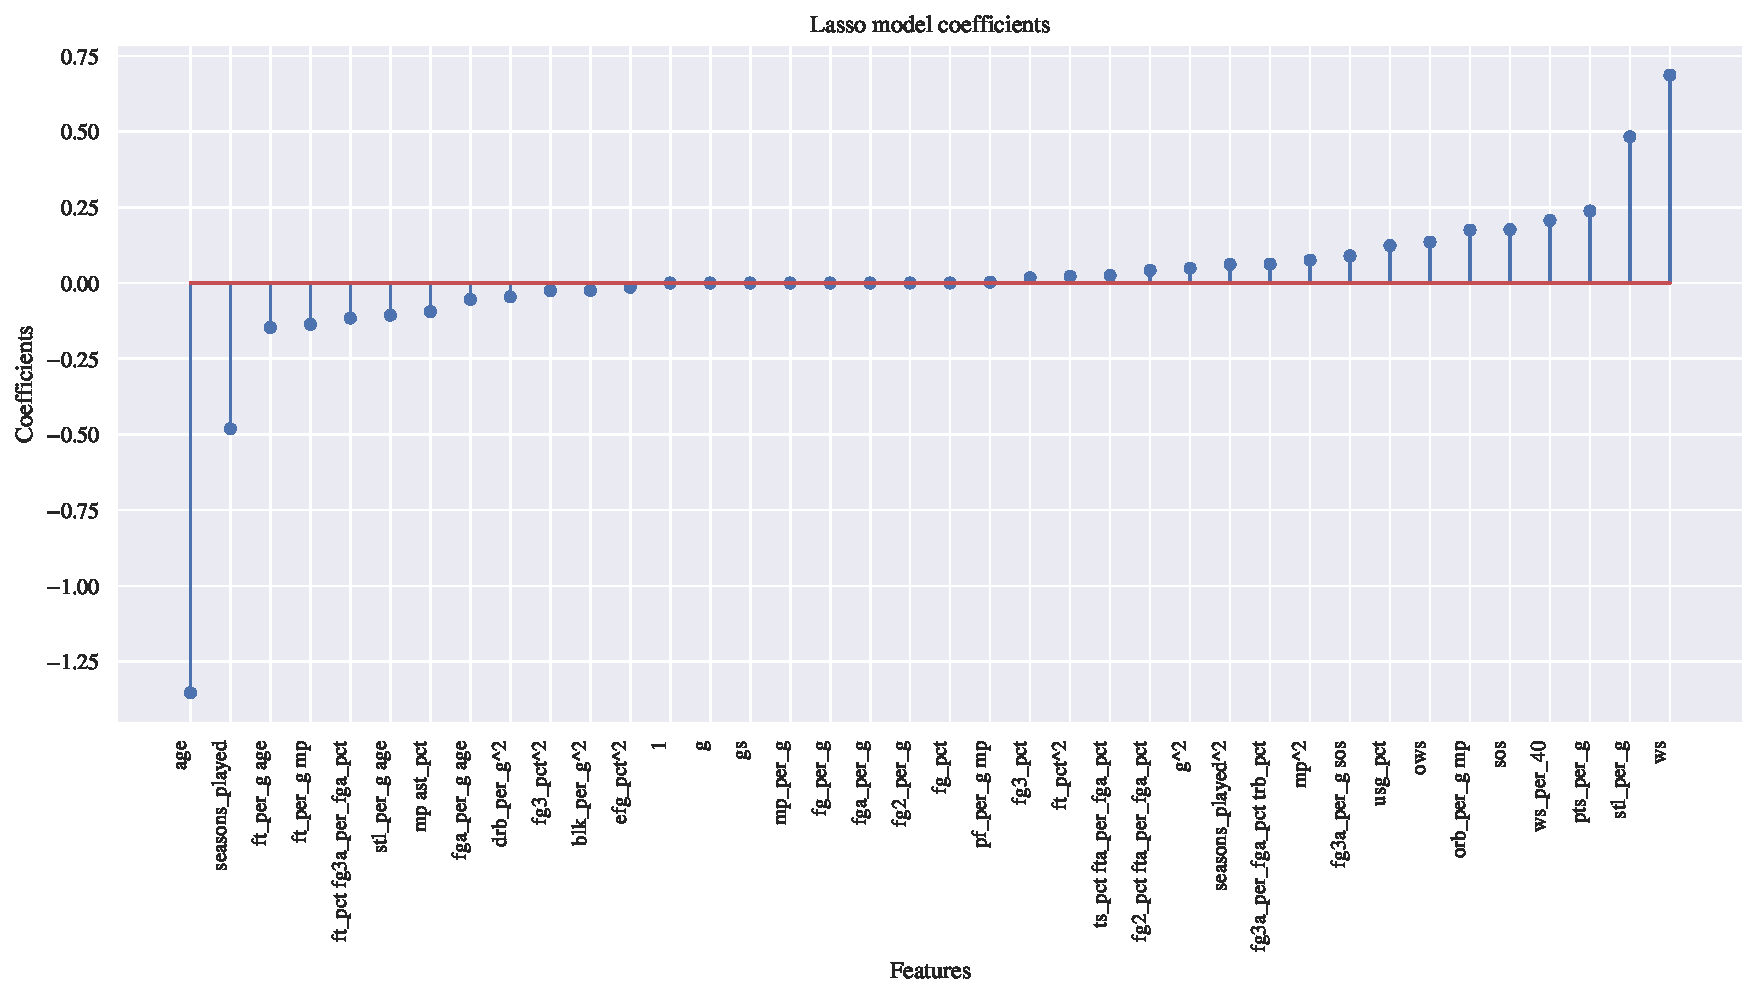
\includegraphics[width=1.0\linewidth]{figures/Lasso_coeffs.pdf}
    \caption{Top Lasso coefficients}
    \label{fig:lasso-coeff}
\end{figure}

\subsection{K-Nearest Neighbors}%
\label{ssub:k-nearest-neighbors}

Before the draft, is it a very common approach for NBA scouts to try to find the NBA player that is most similar to the one they are evaluating. This way, they can have an idea of what to expect. We though KNN could perform great because it works similarly, as it makes its predictions according to the nearest neighbors.

We tried several models with different values of $k$ for weighted and non-weighted versions of knn. Moreover, as knn tends to performance tends to worsen in highly irrelevant feature spaces, we also tried using PCA as a preprocessing step to reduce dimensionality. \Cref{fig:knn} shows the root mean squared error for several configurations. Overall, the best model was a weighted-knn with $k=10$ trained on the top 15 PCA principal components, which obtained 0.02 $R^2$ and 4.87 RMSE.

\begin{figure}[H]
    \centering
    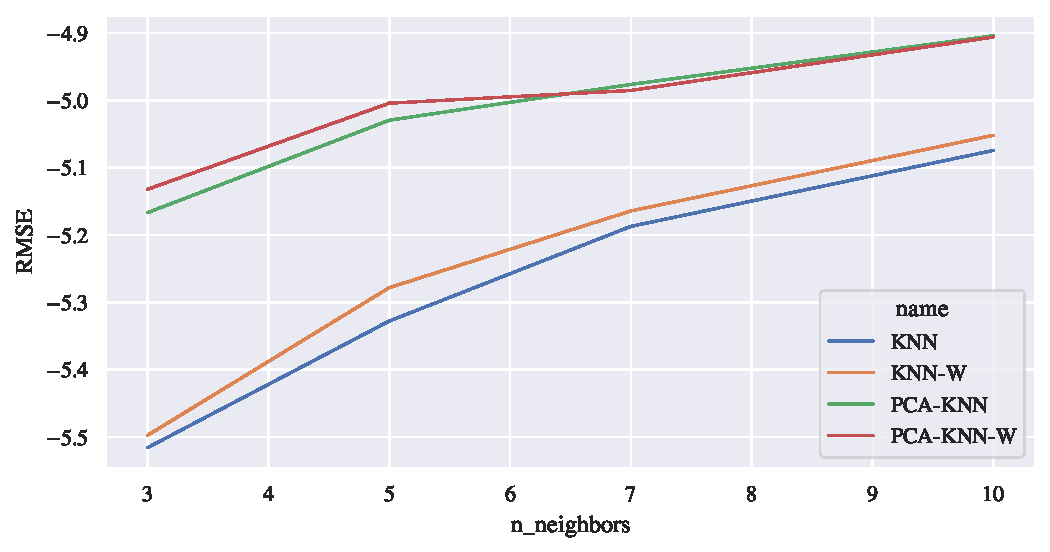
\includegraphics[width=0.7\linewidth]{figures/knn.pdf}
    \caption{Knn plots}
    \label{fig:knn}
\end{figure}

\subsection{Support Vector Machine}%
\label{ssub:support-vector-machine}

We also used Support Vector Regression models. In this case, we tried rbf, sigmoid and polynomial (degree 2,3) kernels and used cross validation to determine a decent value of the penalty hyperparameter ($C$). \Cref{ml:svm} the best performing configuration for each kernel. The best model was an RBF kernel SVM with $C=10$, which obtained 0.2 $R^2$ and 4.35 RMSE.

\begin{table}[H]
    \centering
    \begin{tabular}{lcccccc}
    \toprule
    name & RMSE & $R^2$ & C &  poly\_degree &  epsilon & kernel \\
    \midrule
    SVR-Poly-2 & 4.934976 & & -0.13 & 2.0 &  0.10 & poly \\
    SVR-Poly-3 & 4.653794 & 0.09 & 1.0 & 3.0 & 0.10 & poly \\
    SVR-sigmoid & 4.699737 & 0.06 & 0.1 & NaN & 0.01 & sigmoid \\
    SVR-rbf & 4.357230 & 0.2 & 10.0 & NaN & 0.10 &  rbf \\
    \bottomrule
    \end{tabular}
    \caption{SVM best models}
    \label{ml:svm}
\end{table}

\subsection{Kernel Ridge Regression}%
\label{ssub:kernel-ridge-regression}

\subsection{Ensemble learning}%
\label{ssub:ensemble}

In this section, we will discuss several algorithms that combine multiple base estimators to make the predictions.

\subsubsection{Random Forest}
The first ensemble method we will use is Random Forest which use decision trees as base estimators.  It has many hyperparameters, among which we decided to optimize the 5 following: \texttt{max\_depth}, \texttt{max\_features}, \texttt{n\_estimators}, \texttt{min\_samples\_leaf}, \texttt{criterion} and \texttt{n\_estimators}. Of all configurations, the best model uses 500 estimators, Poisson as split criteria and all features, a max depth of 100 and minimum number of samples to be a leaf of 1.



\subsubsection{AdaBoost}

\subsubsection{Voting}

%   {'criterion': 'poisson',
%   'max_depth': None,
%   'max_features': 'sqrt',
%   'n_estimators': 500})}
